\section{Implementation of Scratch Detector}
In this chapter the development and results of a YOLOv5 solution for detection of scratches found on printed layers of a 3D binder jet printer.
\subsection{Development Environment \& Setup}
Through trial and error the development environment has been continuously improved and finally converged to the one depicted in figure \ref{fig:setup}. A simple dataset manager is used for dataset versioning through FiftyOne's \cite{fiftyone_git} integrated database. Datasets stored in FiftyOne's database can be then visualized in any browser. This helpful for debugging and testing new augmentations methods or visualizing detections and labels in a more interactive way. For annotating labels, CVAT \cite{cvat_git} was one of the more established tools for this task. \\
The augmentation of data can happen in two ways: offline and online. Ideally is to have as many online augmentations as possible, but the online augmentation framework provided by YOLOv5 forces that each augmentation method takes as input a exactly one labeled image and outputs exactly one labeled image. Changing this framework to be flexible to more output images is difficult, since the underlying albumentations library \cite{albumentations_site} works on the same one input-one output principle. Therefore, for those type of augmentations method is best to be made offline and this is the task of the \textit{Augmenter} from the figure. \\
For logging Weights \& Biases \cite{wandb_site} was a good candidate, because it's feature rich and YOLOv5 has native support for this. YOLOv5 supports also Tensorboard and ClearML.\\

 \begin{figure}[!h]
  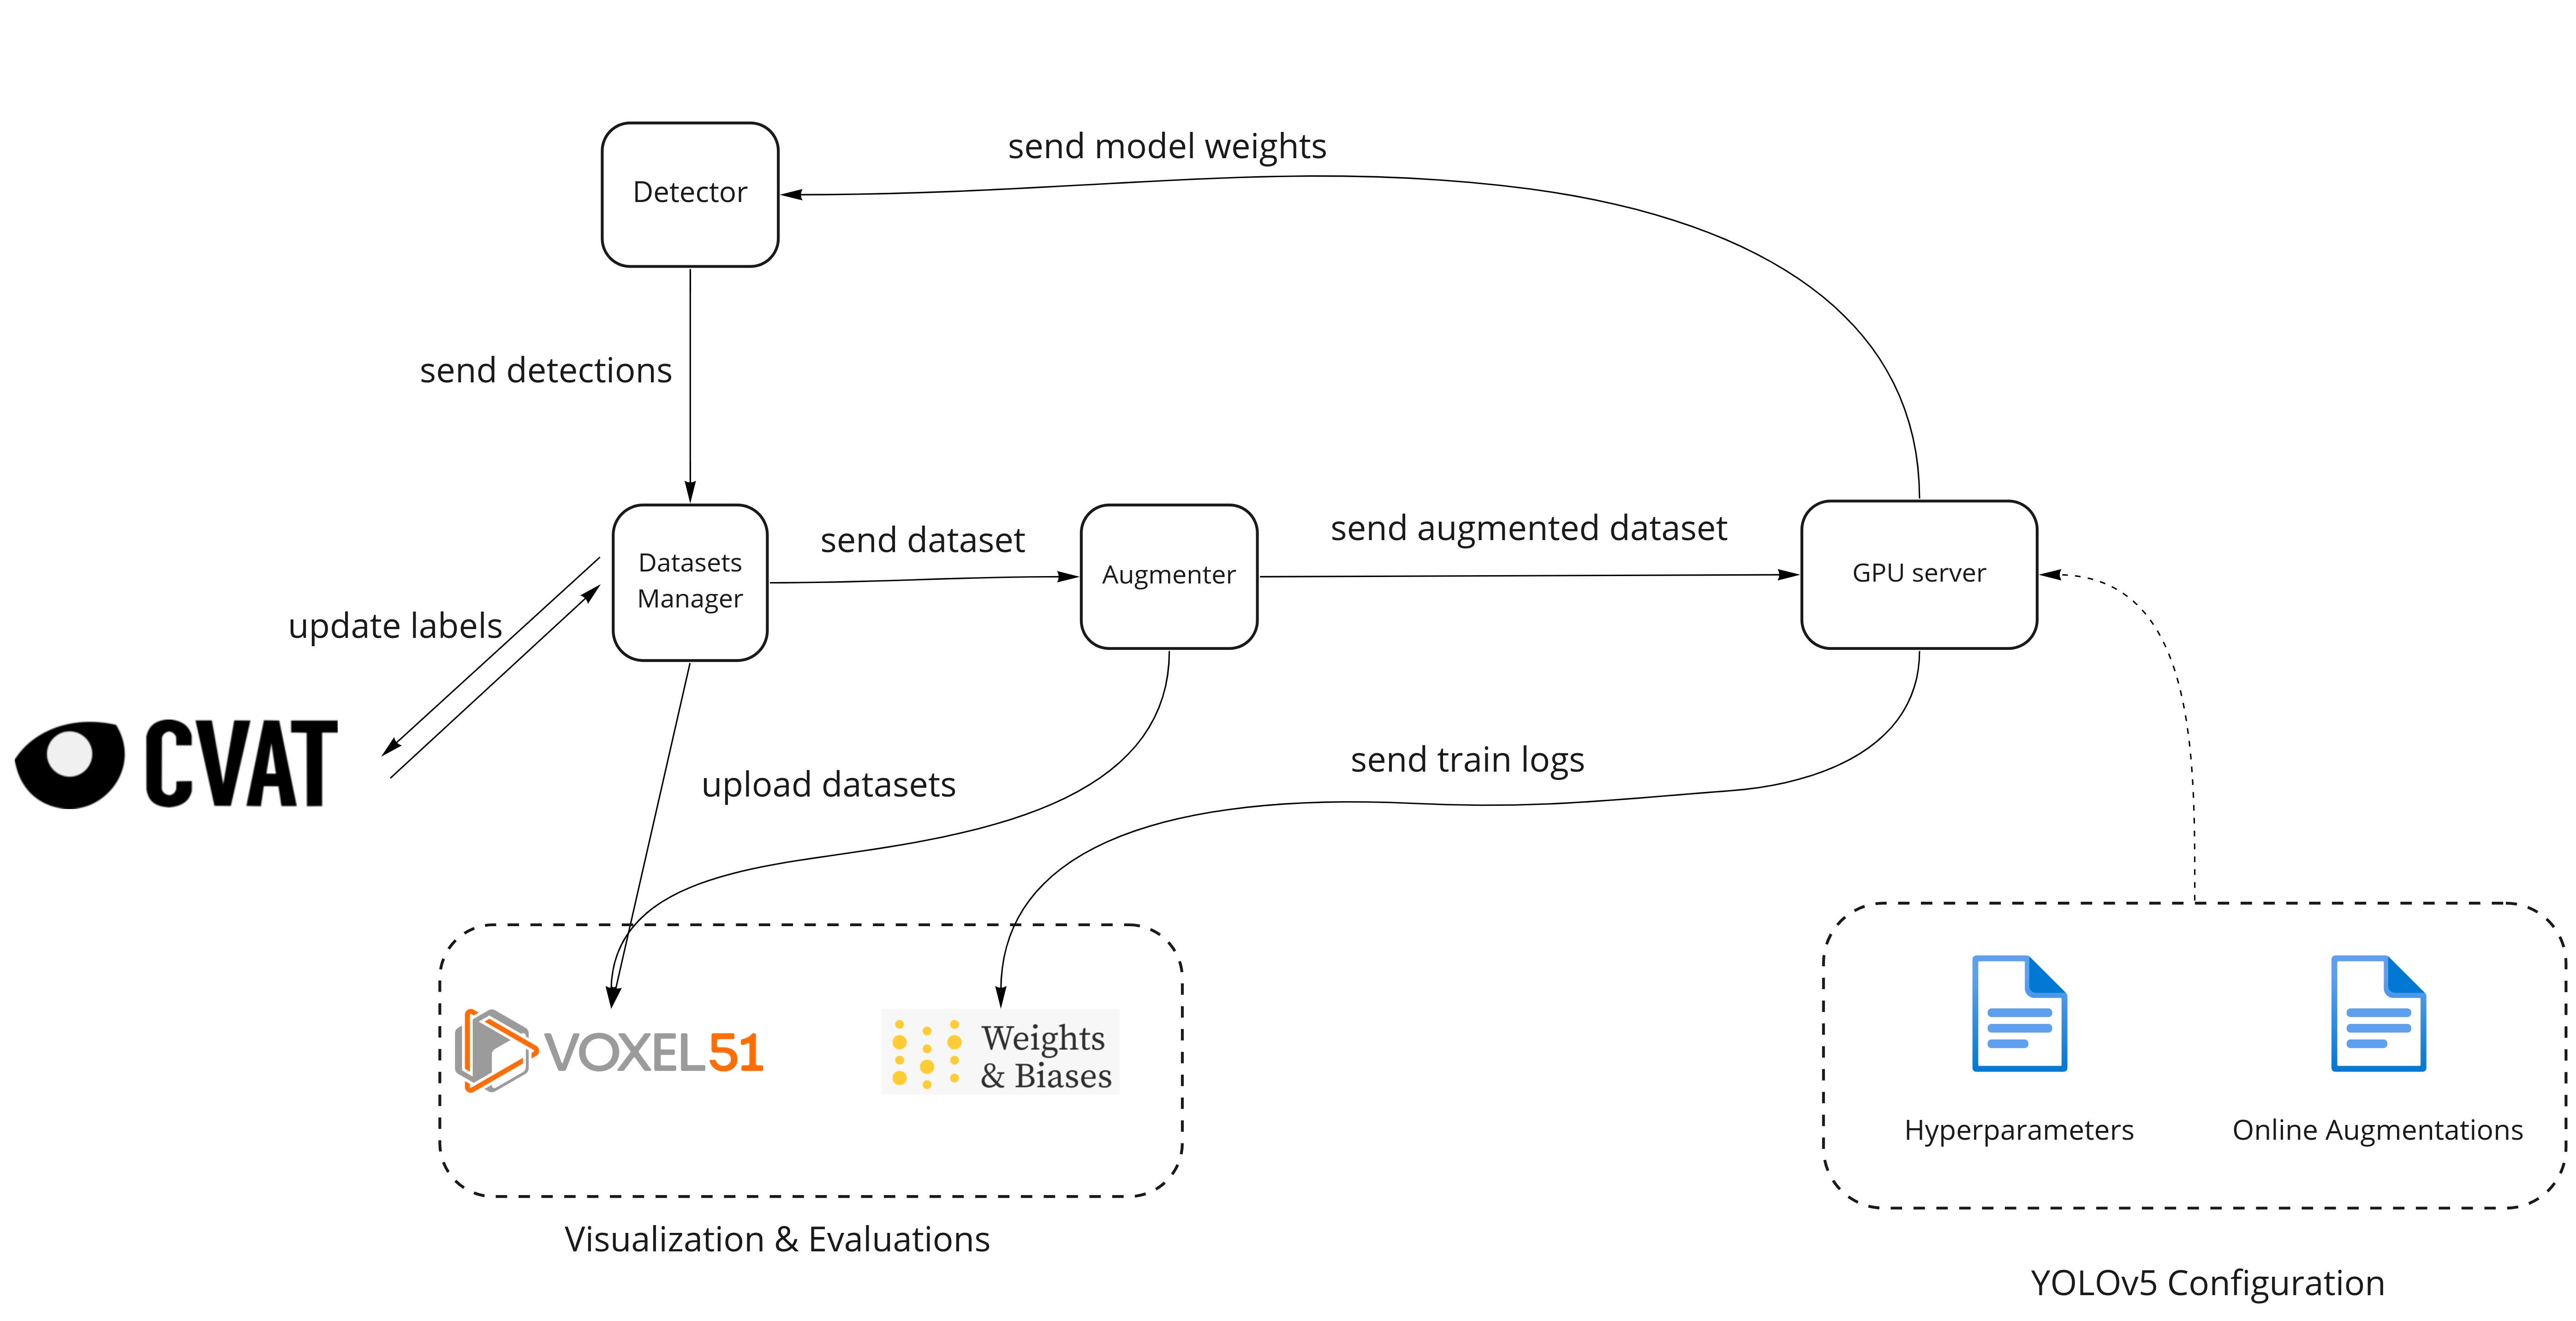
\includegraphics[width=\textwidth]{images/setup}
  \caption{title}
  \label{fig:setup}
\end{figure}

For detection the \textit{detector.py} script provided in YOLOv5 can be used, but an official detector can also be loaded from PyTorch Hub. The latter solution is better for post processing detections.

\subsection{Annotation}
Annotating the dataset was a tougher challenge than anticipated, because it's not always clear if the dark line is a scratch, thin split in the component or some artifact visible from the layer before. \\

\begin{figure}[ht]
  \centering

  \begin{subfigure}{\textwidth}
    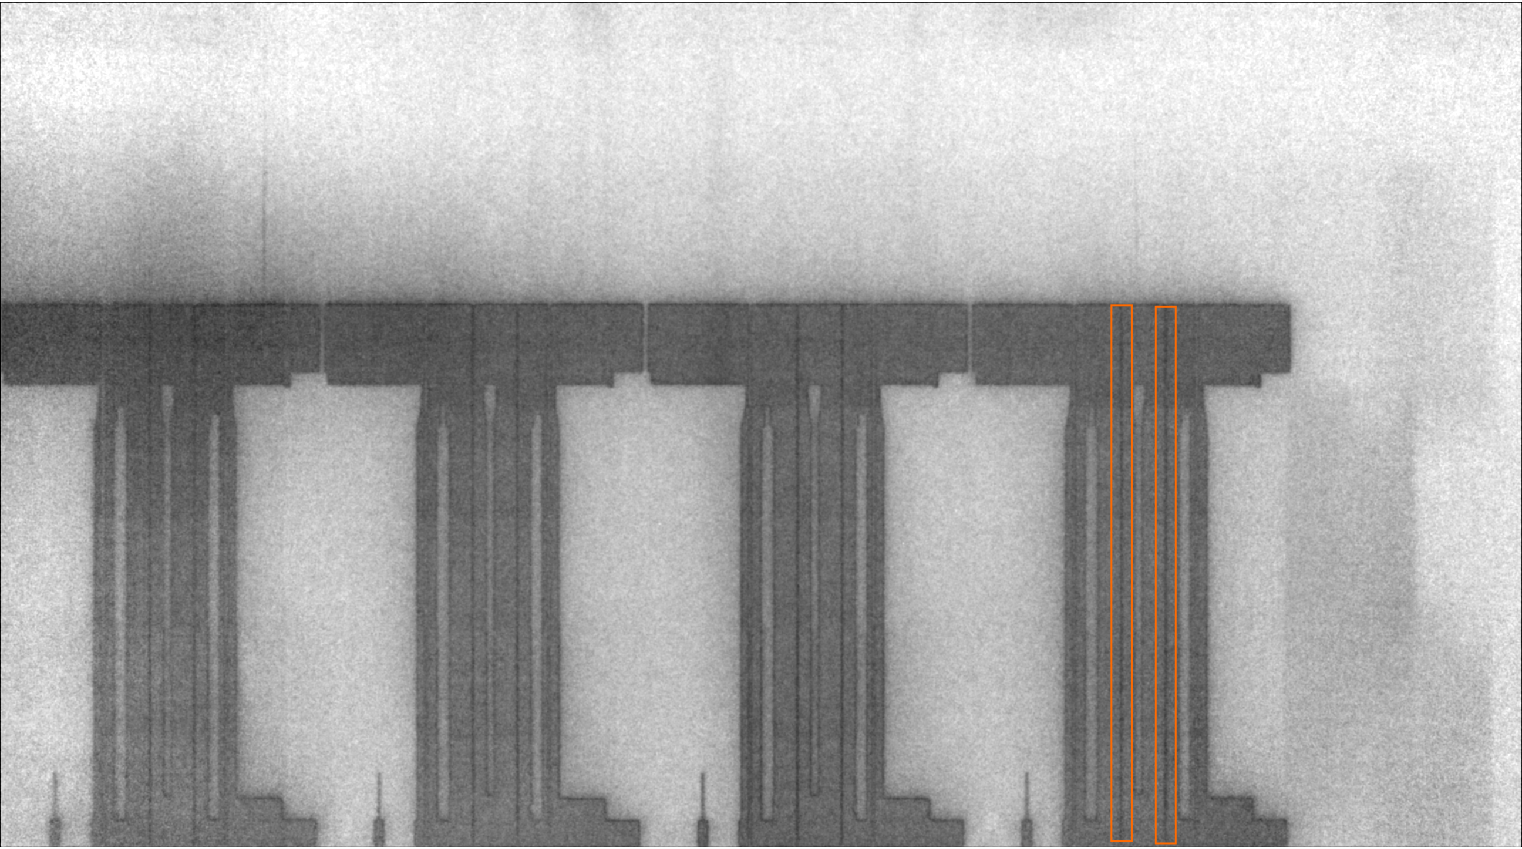
\includegraphics[width=\textwidth]{images/layer_01486_marked}
    \caption{Layer with thin splits marked in orange bounding boxes.}

  \end{subfigure}

  \begin{subfigure}{\textwidth}
    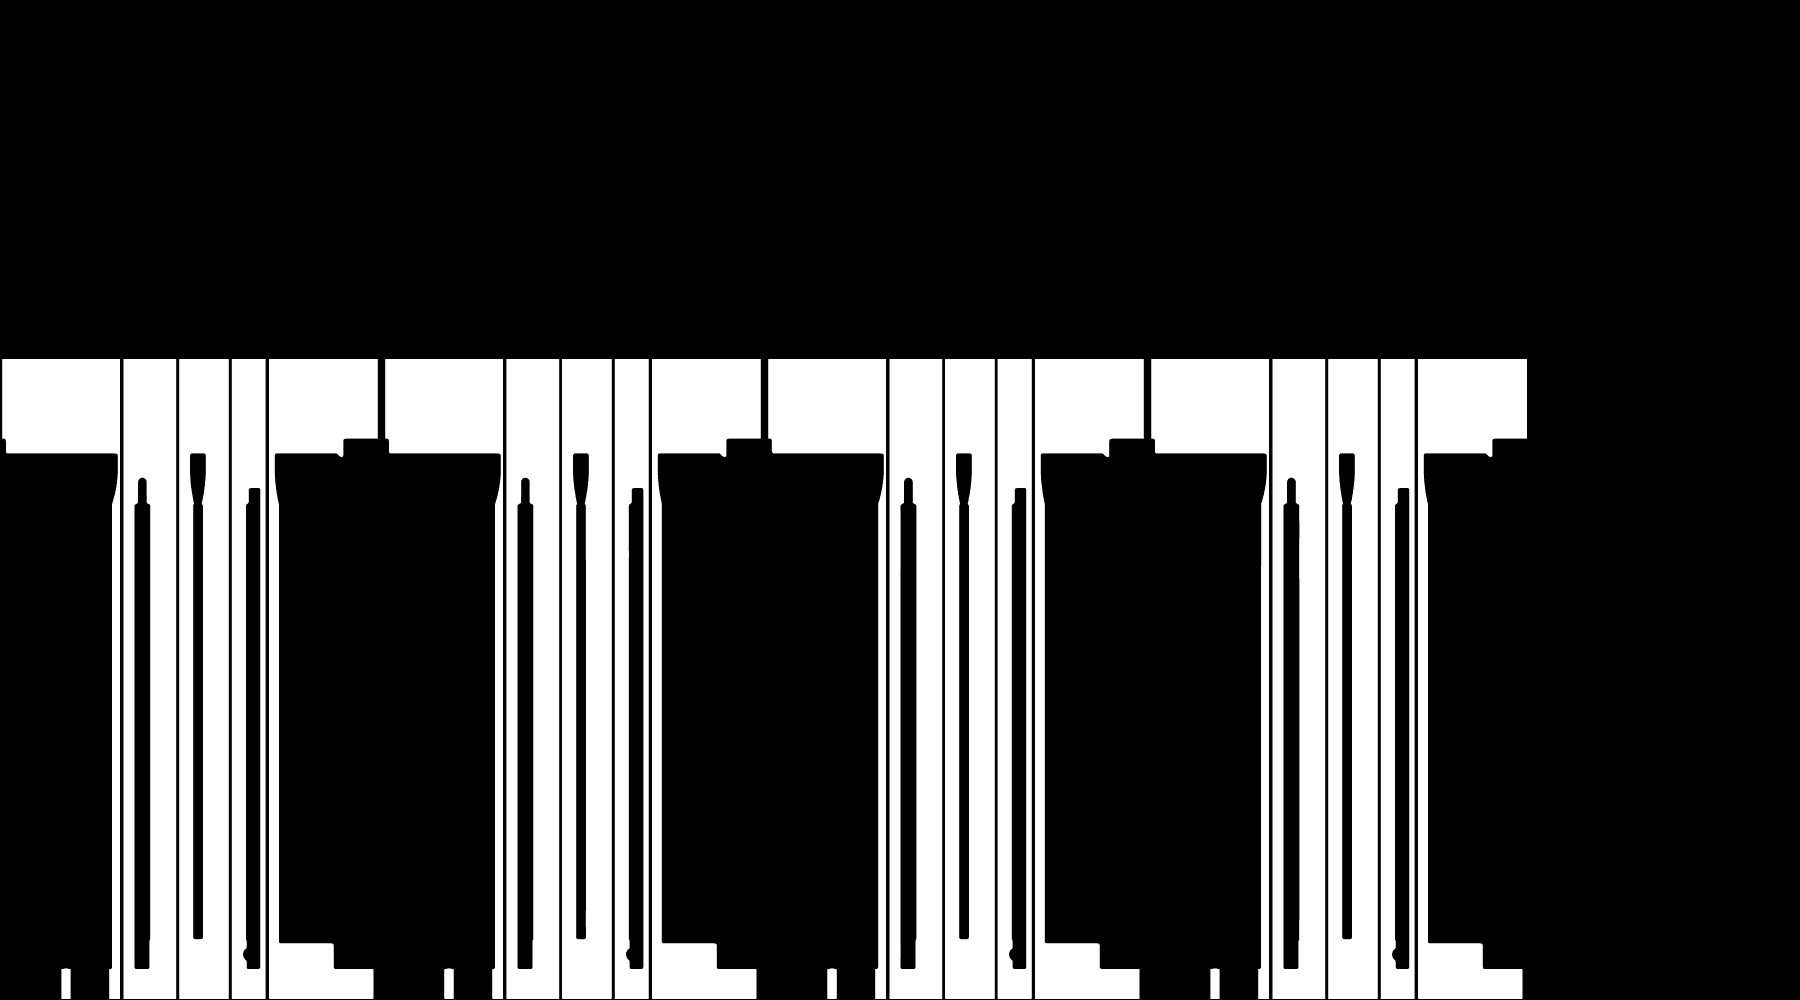
\includegraphics[width=\textwidth]{images/bitmask_01486}
    \caption{Corresponding bitmask must be checked to see if it's a scratch or a thin split.}
  \end{subfigure}

  \caption{Thin splits}
  \label{fig:layer_01486}

\end{figure}

The safer, but more tedious route is to check layer by layer the corresponding bitmask. This is only one of the many things to consider when annotating.\\

Sometimes the scratch is also barely visible or one cannot be sure if the scratch is relevant. Adding every fine scratch will make the model oversensitive, leading to many false positive. One statistical way to determine the strength of a labeled scratch goes roughly as follows:
\begin{enumerate}
\item Crop from the layer a window outlined by the bounding box.
\item Calculate the sum of rows of the image into a vector.
\item Multiply by -1 the whole vector.
\item Treat the vector as a signal and calculate prominences for the peak.
\item Multiple the prominence by a constant scaling factor.
\end{enumerate}

This way the bounding box is converted to signal, which makes a analysis of the strength of the scratch a bit more deterministic. After the 3rd step the plotted vector should look like this:

\begin{figure*}[!h]
\begin{center}
        \begin{subfigure}{0.3\textwidth}
        \centering
        
\includegraphics[width=0.2\textwidth]{images/crop_bb}
        \caption{Cropped bounding box}
    \end{subfigure}
                \quad
    \begin{subfigure}{0.55\textwidth}
        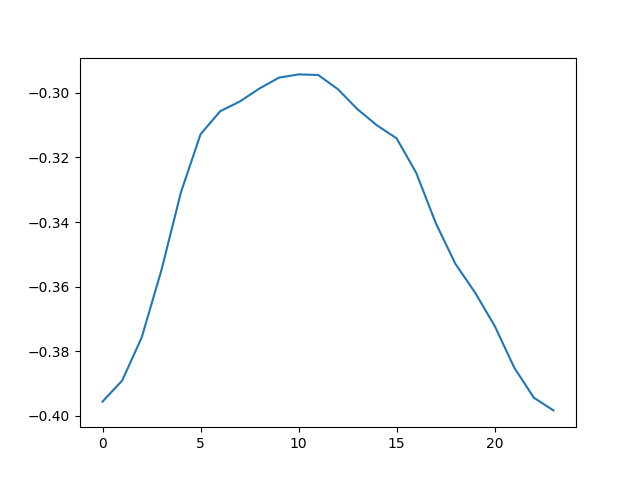
\includegraphics[width=\textwidth]{images/signal_bb}
        \caption{Bounding box signal}
    \end{subfigure}
            \quad

\caption{TODO: align images.  Transforming a bounding box to a signal.}
\label{default}
\end{center}
\end{figure*}

This method forces the annotation process to be more consistent, but it should be treated as statistical process and not as a deterministic one. In figure \ref{fig:prom_ex} can be seen why this process should not be seen as deterministic: the two scratches are of similar visibility, but have very different prominence values. Luckily, such outliers were rare. \\
One nice trick to visualize the scratches with the respective prominence value was to create a copy of the existing ground truth dataset and transform the ground truth labels to detections and as confidence value to use the prominence value. Note that in YOLOv5 the only difference between a ground truth bounding box and detection is that the detection has the optional confidence value filled out or less than 1.0. TODO: refer to the chapter that discusses labels (and also update that chapter) \\

\begin{figure}[!h]
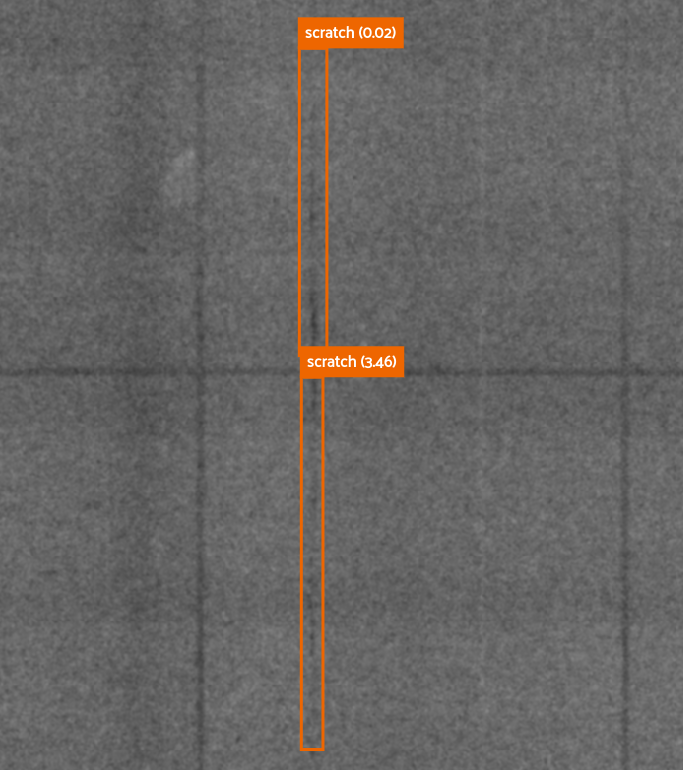
\includegraphics[width=\linewidth]{images/prominence_example}
\caption{Scratches with prominence values.}
\label{fig:prom_ex}
\end{figure}

Another problem are artifacts, that come from previous layers. Some cases are easy to recognize, but a common tricky situation is, if thin splits from previous layers are visible on the current layer. In those situations the thin splits might look like a scratch, have an acceptable prominence value and the bitmask indicates that in the respective region is no thin split. Therefore, the only way to really determine, if it's a scratch or not, is to analyze the previous layer too. As one can see, the annotation process got even more tedious, which means that data gathering is time-consuming and/or expensive.
TODO: say later we will see data cost table \\

\begin{figure*}[!h]
\begin{center}
        \begin{subfigure}{0.6\textwidth}
        \centering
        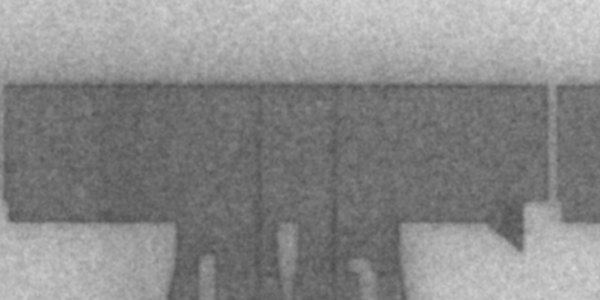
\includegraphics[width=\textwidth]{images/thin_scratch_previous_layer/layer_00107}
        \caption{A layer with dark lines}
    \end{subfigure}
                \quad
    \begin{subfigure}{0.6\textwidth}
        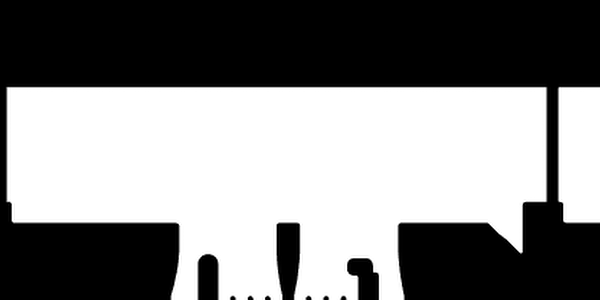
\includegraphics[width=\textwidth]{images/thin_scratch_previous_layer/bitmask_00107}
        \caption{Current bitmask has no splits.}
    \end{subfigure}
    \begin{subfigure}{0.6\textwidth}
        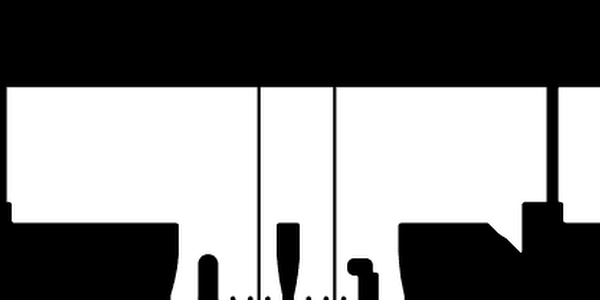
\includegraphics[width=\textwidth]{images/thin_scratch_previous_layer/bitmask_00106}
        \caption{Previous bitmask contains the seen splits.}
    \end{subfigure}
            \quad

\caption{Example of how thin splits are actually from the previous layer.}
\label{fig:thin_splits_previous_layer}
\end{center}
\end{figure*}


\subsection{Augmentation Pipeline}
TODO: muss ich sagen woher ideal dataset? \\
The dataset at hand features a total of 2295 images of layers with the corresponding bitmask, but only a fraction of the images contain an actual scratch. This makes the dataset from the recommended minimum of 1500 images per class and 10000 instances per class. This forced a focus shift on augmentation methods. \\
When it came to evaluating an augmentation method, identical dataset shuffles (train, validation, test splits) were used for multiple reasons. One reason is that it's easier to visually compare the validation errors, if the exact same image is used. One nice feature supported with Weights \& Biases logger is the Bounding Box Debugger, which lets the user see the validation labels for each epoch for multiple runs. If the runs had the exact same validation images, then a head-to-head comparison was possible.\\

\begin{sidewaysfigure}
    \centering
    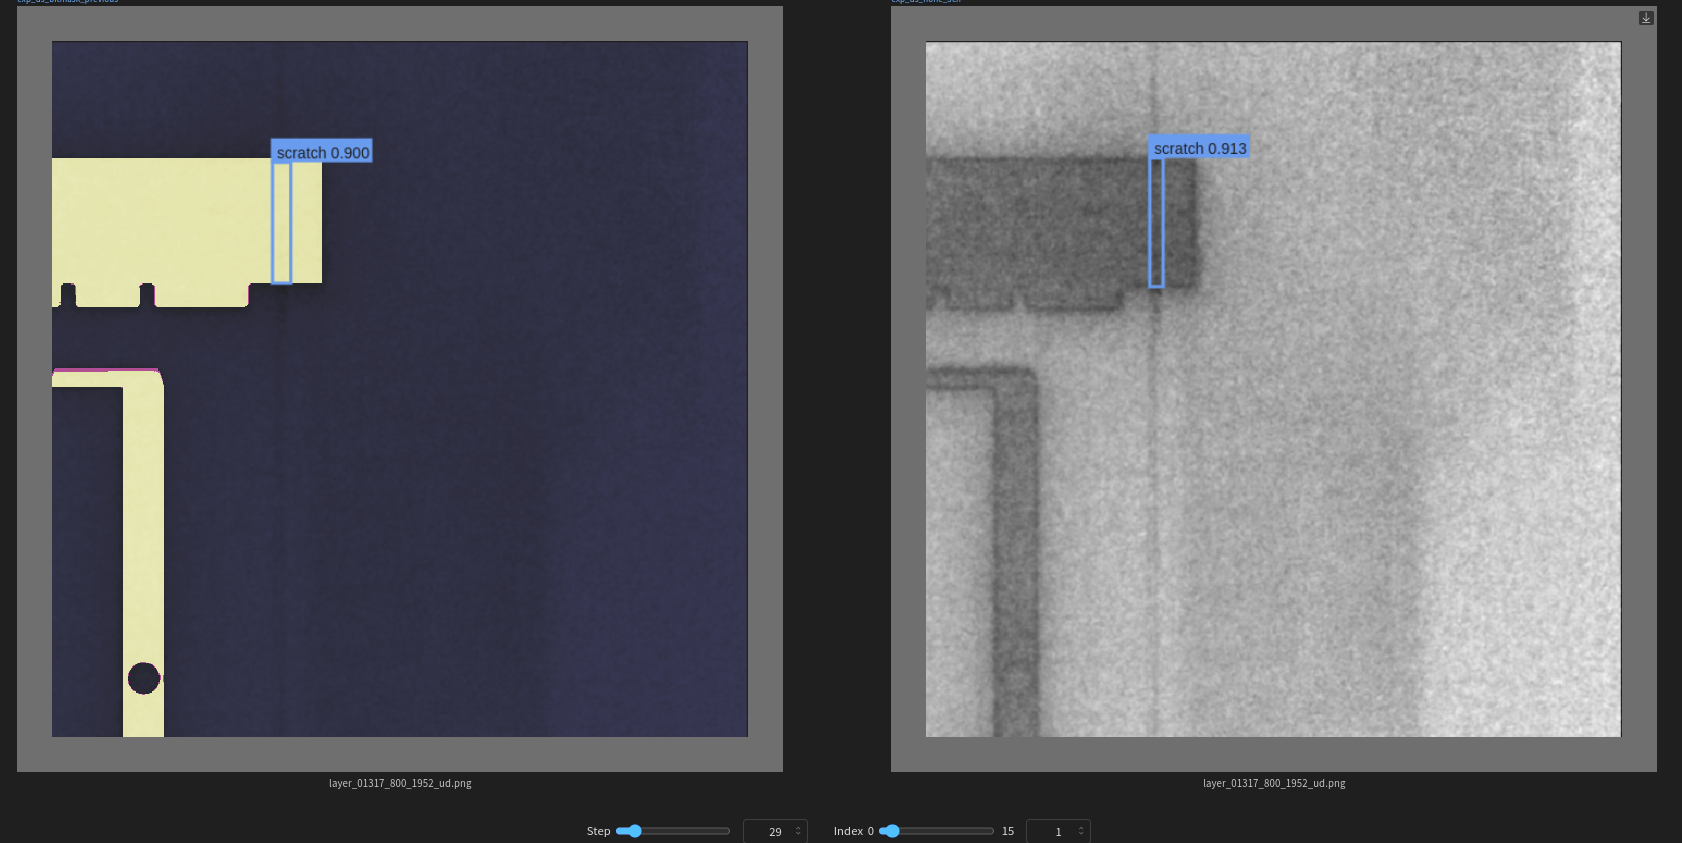
\includegraphics[width=\textwidth]{images/bb_debugger}
    \caption{Comparing head-to-head detections on validation images with the Bounding Box Debugger}
    \label{fig:bb_deb}
\end{sidewaysfigure}

Another reason for using identical shuffles is that in small datasets, shuffles are game of chance in terms of data variety. So, when using an identical shuffle, the same variety is ensured. TODO: maybe delete or reformulate this. \\
